\section{Filterbanken}
Filterbanken teilen das Frequenzspektrum in Teilb�nder auf. Sie arbeiten mit
symmetrischen Hoch und Tiefp�ssen. Im folgenden sind drei g�ngige Strukturen
aufgezeigt, welche den Analyseteil beschreiben. Werden diese Strukturen
gespiegelt, kann das Signal wieder rekonstruiert werden (Synthese).\\
\begin{minipage}[t]{6cm}
	\textbf{Baumstruktur}\\
	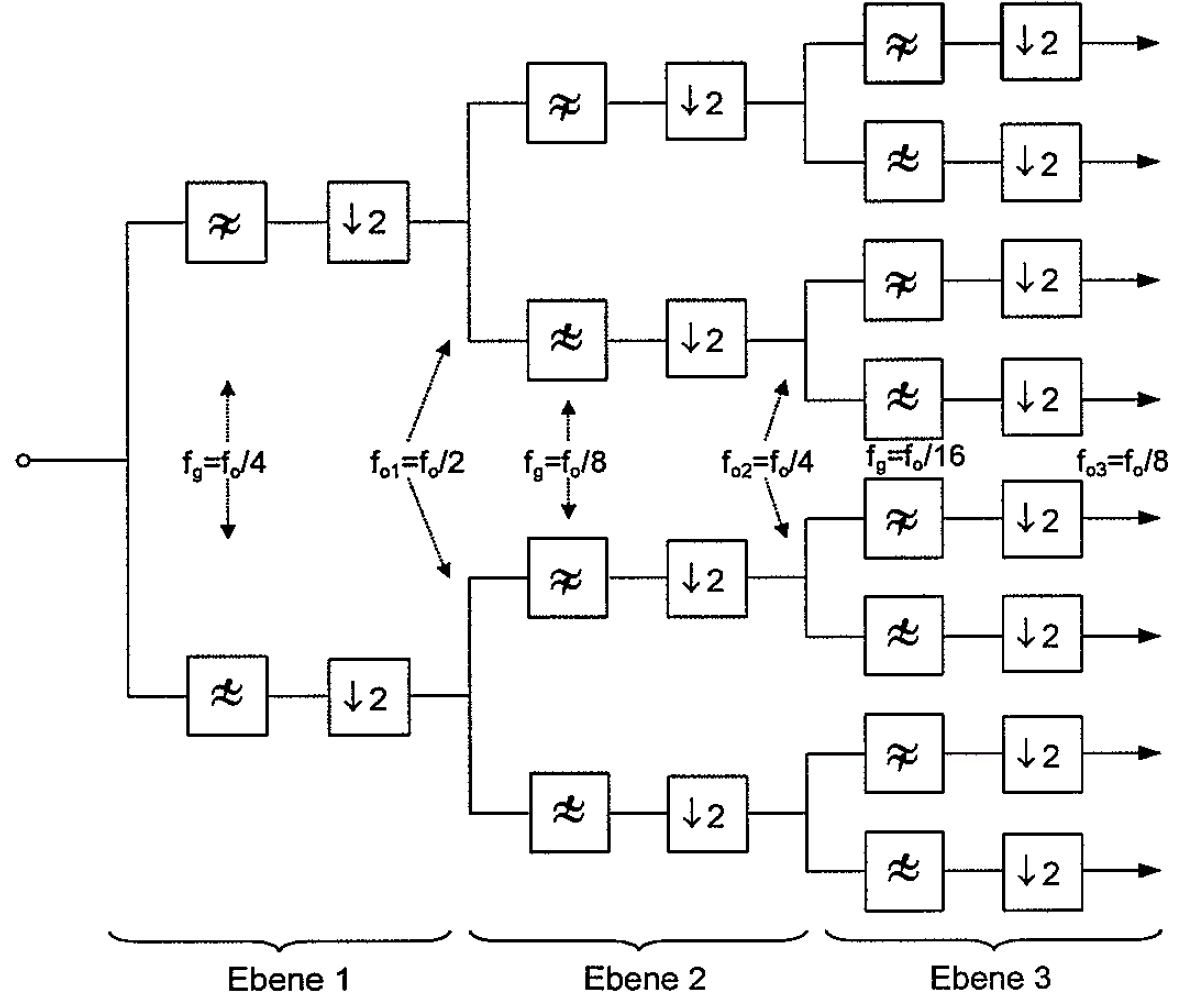
\includegraphics[width=5.8cm]{Content/Filterbanken/Filterbanken_1.PNG}	
\end{minipage}
\vspace{0.1mm}
\hfill
\begin{minipage}[t]{12.5cm}
	\begin{minipage}[t]{6cm}
		\textbf{Parallelstruktur}\\
		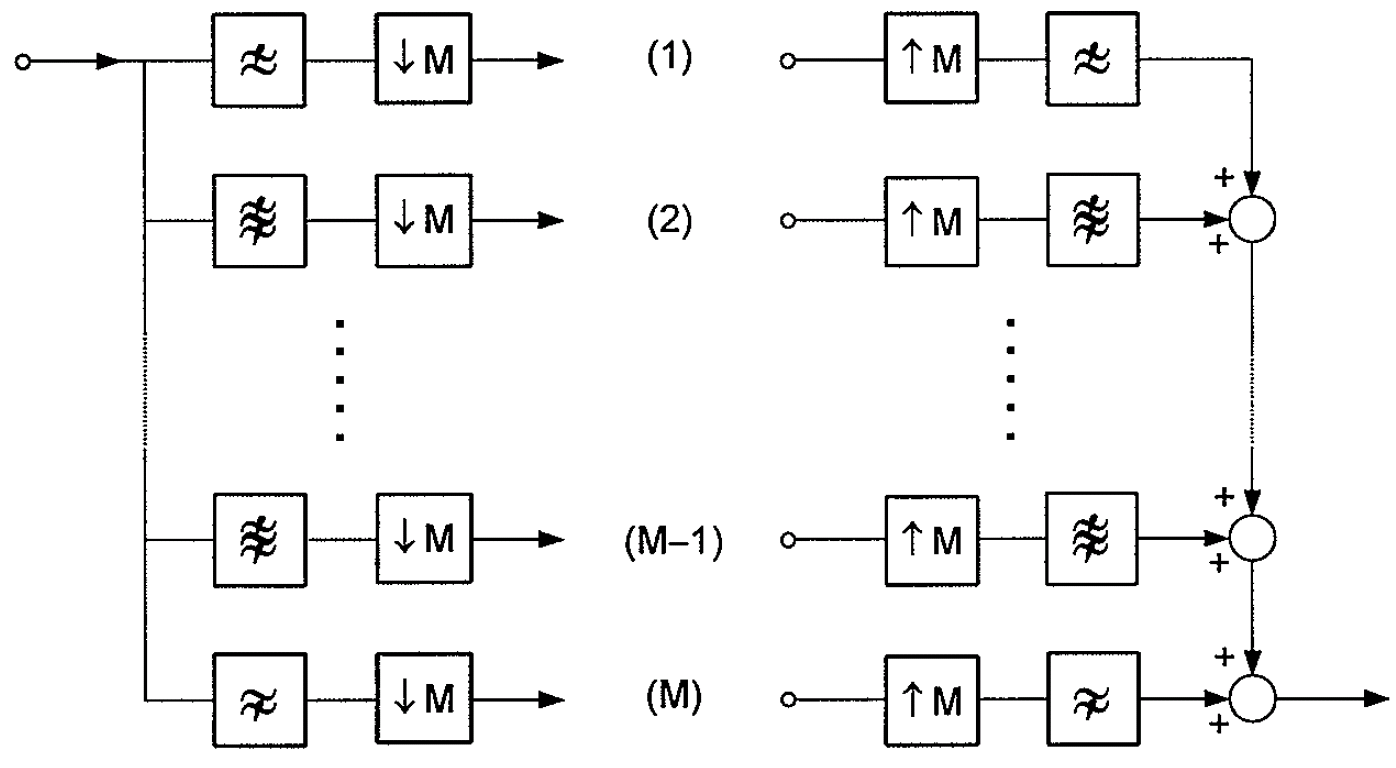
\includegraphics[width=6cm]{Content/Filterbanken/Filterbanken_2.PNG}	
	\end{minipage}
	\hfill
	\begin{minipage}[t]{6cm}
		\textbf{Oktavstruktur}\\
		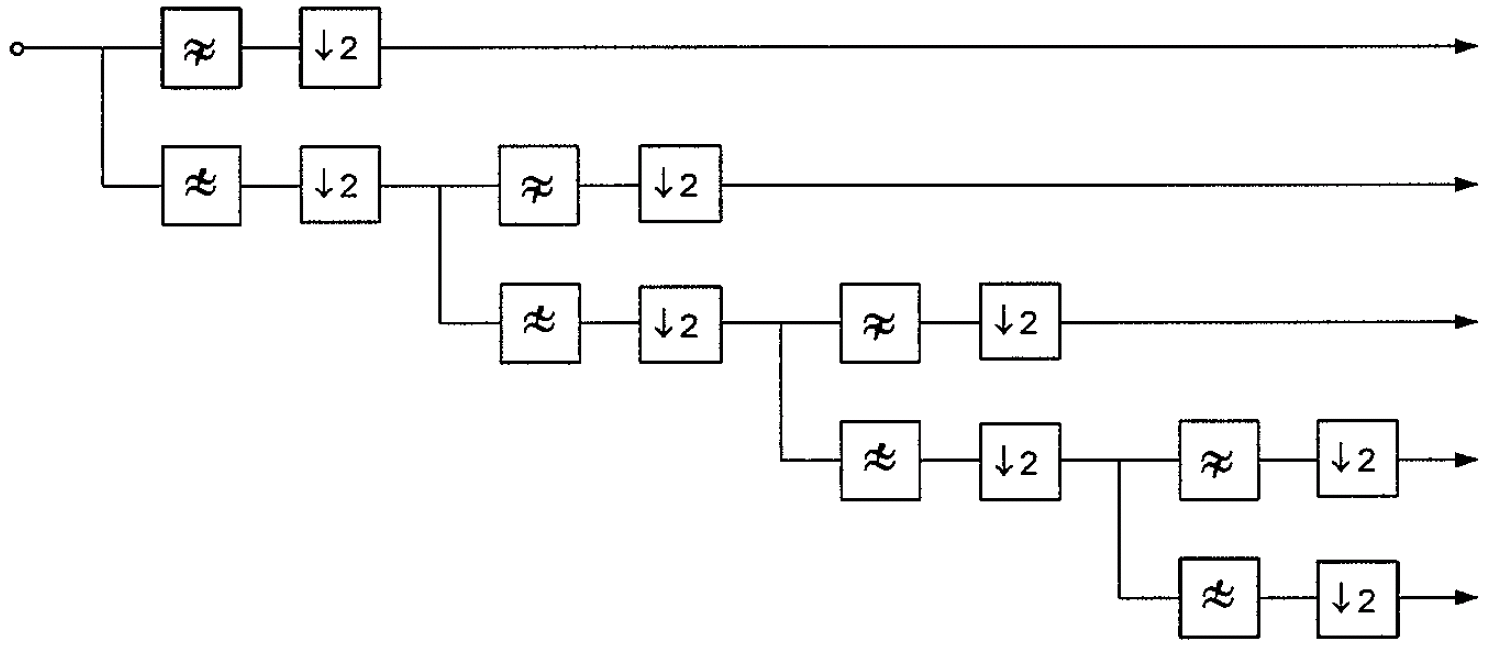
\includegraphics[width=6cm]{Content/Filterbanken/Filterbanken_3.PNG}\\
		Wird f�r die Wavelettransformation eingesetzt	
	\end{minipage}
	\hfill
	\begin{minipage}[t]{4.5cm}
		\textbf{Praktische Beziehungen}\\
		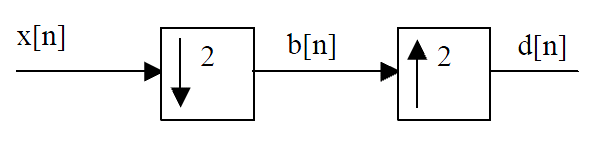
\includegraphics[width=4.5cm]{Content/Filterbanken/Filterbanken_4.PNG}
	\end{minipage}
	\hfill
	\begin{minipage}[t]{7.5cm}
		\vspace{2mm}
		%\small%\scriptsize
		$B(z)=0.5(X(\sqrt{z})+X(-\sqrt{z}))$\\
		$D(z)=B(z^2)=0.5(X(z)+X(-z))$
	\end{minipage}
\end{minipage}